\documentclass[12 pt]{article}
\usepackage[left=2.66cm,top=3cm,right=2.66cm,bottom=3cm,bindingoffset=0.5cm]{geometry}

\usepackage{graphicx}
\usepackage{setspace}
\usepackage{hyperref}
\usepackage{enumitem}
\onehalfspacing

\begin{document}
	
	\begin{center}
		
		\begin{Huge}
		\textbf{HCCO}
		\end{Huge}
			
		\begin{Large}
		\textsc{IN INTERSTELLAR SPACE\linebreak}
		\end{Large}
		
		\begin{scriptsize}
		$
		\textsc{Divya Raj }\bullet\textsc{ David Nallapu }\bullet\textsc{ Simran Srivastava }\bullet\textsc{ Anushree Avasthi }\bullet						\textsc{ Bhavya Aggarwal}	
		$
		\end{scriptsize}
				
	\end{center}
	
	\section*{Structure}
		The  ketenyl  radical(HCCO) has  a  planar  structure  with  a  practically  linear  CCO  backbone  and  the  H  atom  lying  out  of  			the	linear  axis.  The  radical  has a ${}^2A''$ ground  electronic  state  and a  complex  rotational  structure  whose $N_{K_a,K_c}$ 			levels  split in  a	fine (electronic spin-rotation interaction) and hyperfine (H nuclear  spin)  structure  described  by  the  quantum  		numbers J and F, respectively.
		
		\begin{figure}[h!]
		  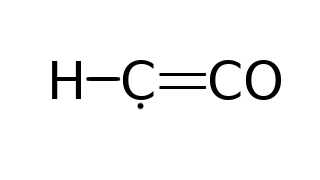
\includegraphics[width=50mm]{hcco.png}
  			\centering
  			\caption{The Ketenyl radical, Lewis structure }
  			\label{fig:PublicKey-Basic}
		\end{figure}
		
	\section*{Interstellar Sources of Detection}
		HCCO was first detected in the starless core Lupus-1A and the molecular cloud L483.\cite{mcg}
		
	\section*{Observation Techniques}
		The observation which led to the discovery of the molecule in interstellar space were ground based and were carried out using the
		\href{https://en.wikipedia.org/wiki/IRAM_30m_telescope}{IRAM 30m}
		millimeter radio telescope, \\located in Veleta, Granada Province, Spain.\cite{IRAMwiki}
		\\\\The observations were made in selected frequency ranges from 83 to 105 GHz, which fall under the Ultra high microwave frequency 
		range.\cite{EMwiki}
		\\The spectrum of Lupus-1A around 86.65 GHz showed a quartet of emission lines whose frequencies coincide precisely with the	
		strongest fine and hyperfine components of the $N=4-3$ rotational transition of the HCCO radical\cite{mcg}
		
	\section*{Formation Mechanism}
		The main formation  route  to  HCCO  is  the  reaction  between  $OH$  and  $C_{2}H$.
		This reaction is exothermic and has an estimated rate constant
		of $3\times10^{11}cm^3s^{-1}$.
		\begin{center}
		$OH + C_2H \rightleftharpoons HCCO + H $
		\end{center}
		The reaction between  atomic  O  and  $C_2H_2$	is  also  exothermic  in  the  channel yielding HCCO, although its reaction barrier 				is too large to be relevant at low temperatures.
		\begin{center}
		$O + C_2H_2 \rightleftharpoons HCCO + H $
		\end{center}
		A possible precursor of HCCO is ketene. The reaction of ketene with OH is a potential source of HCCO radicals because this 						reaction is rapid, although it seems to have a low yield of HCCO.
		The HCCO radical reacts readily with neutral atoms and molecules present around it. It does so at a faster rate than its estimated rate 		due to the above mechanisms.Hence, A  powerful  formation  mechanism  of  HCCO  is  needed  to counterbalance  the  efficient  					depletion  of  this  radical  by  reactions  with  neutral  atoms.\cite{mcg}  An  interesting  possibility is the reactions of O 							atoms with $C_nH$ radicals $(n>3)$, which are assumed to yield CO because this is the most exothermic channel, although the 						channel leading to HCCO is  also  exothermic.  It  is  also  worth  noting  that  recent  studies find that ketene can
		be  efficiently  formed  in  various  types  of  ices  upon  irradiation with energetic electrons and ultraviolet photons (both of 				which can  be  formed  in  dark  clouds  following  cosmic-ray  impacts), which  opens  the  possibility  to  the  formation  of  HCCO  		as  an intermediate.
				
	\begin{thebibliography}{999}
	\bibitem{mcg}
 	 Marcelino Agúndez, José Cernicharo, and Michel Guélin, \emph{Discovery of interstellar ketenyl (HCCO), a surprisingly abundant radical}.
 	 April, 2015.
	
	\bibitem{IRAMwiki}
	Wikipedia - \href{https://en.wikipedia.org/wiki/IRAM_30m_telescope}{IRAM 30m telescope}
	
	\bibitem{EMwiki}
	Wikipedia - \href{https://en.wikipedia.org/wiki/Electromagnetic_spectrum}{Electromagnetic Spectrum}	
	\end{thebibliography}
	
\end{document}
